\chapter[2021 June]{June 2021}

\section[2021/06/11]{Friday, 11 June 2021}

\subsection{Centroid Detection for Multiple Cubes}

Previous results have shown that segmentation of the top face of the cube based on light intensity offers the most promising avenue to robustly detect and localise the cube. In order to develop this concept further, several adjustments were made to the previous image processing test setups. Firstly, it was previously demonstrated that the introduction of colour information into the image through the addition of a coloured background offers no better performance than pure light intensity information. Therefore, in order to maximise the light intensity differential between the reflective top face of the cube, a plain matte black paper background was introduced. Secondly, it was observed that when the angle between the light incident on the top face of the cube and the light reflected into the camera is minimised, the light intensity on the top face of the cube as observed by the camera is maximised. To make the most of this effect, the camera was placed parallel to the base plane at a height of approximately 500 mm with two bright \ac{LED} lights on either side angled toward the centre of the base plane. Lastly, to test that the ability of the image processing algorithm to detect multiple cubes in the same image with variying top face light intensities, multiple cubes were placed randomly on the base plane.

\FigRef{fig:multiple-cubes} shows the image that was captured with the above setup. Note the light intensity on the top face of each cube. The first step in extracting the contours from the image is to apply binary thresholding to the image to segment the top faces of the cubes. In preparation for this, the image was first converted to grayscale and blurred. The binary threshold in which only pixels with intensities greater than 140 out of 255 were retained. This resulted in a well segmented collection of cube top faces. The OpenCV contour detection algorithm was then applied to this binary images which resulted in the red contours shown in \FigRef{fig:multiple-cube-centroids}. Finally, the moment of each contour was calculated and used to find the centroid of each face. These centroids are indicated as blue dots in \FigRef{fig:multiple-cube-centroids}. All the cube centroids were successfully detected in terms of the image coordinate system which is sufficient output from the object detection phase. Methods to attain the vertices of the upper face will still be explored with the intent of use in pose estimation. The next process to be investigated needs to be capable of mapping these image coordinates to the world coordinate system.

\begin{figure}[H]
    \centering
    \begin{subfigure}[b]{0.45\textwidth}
         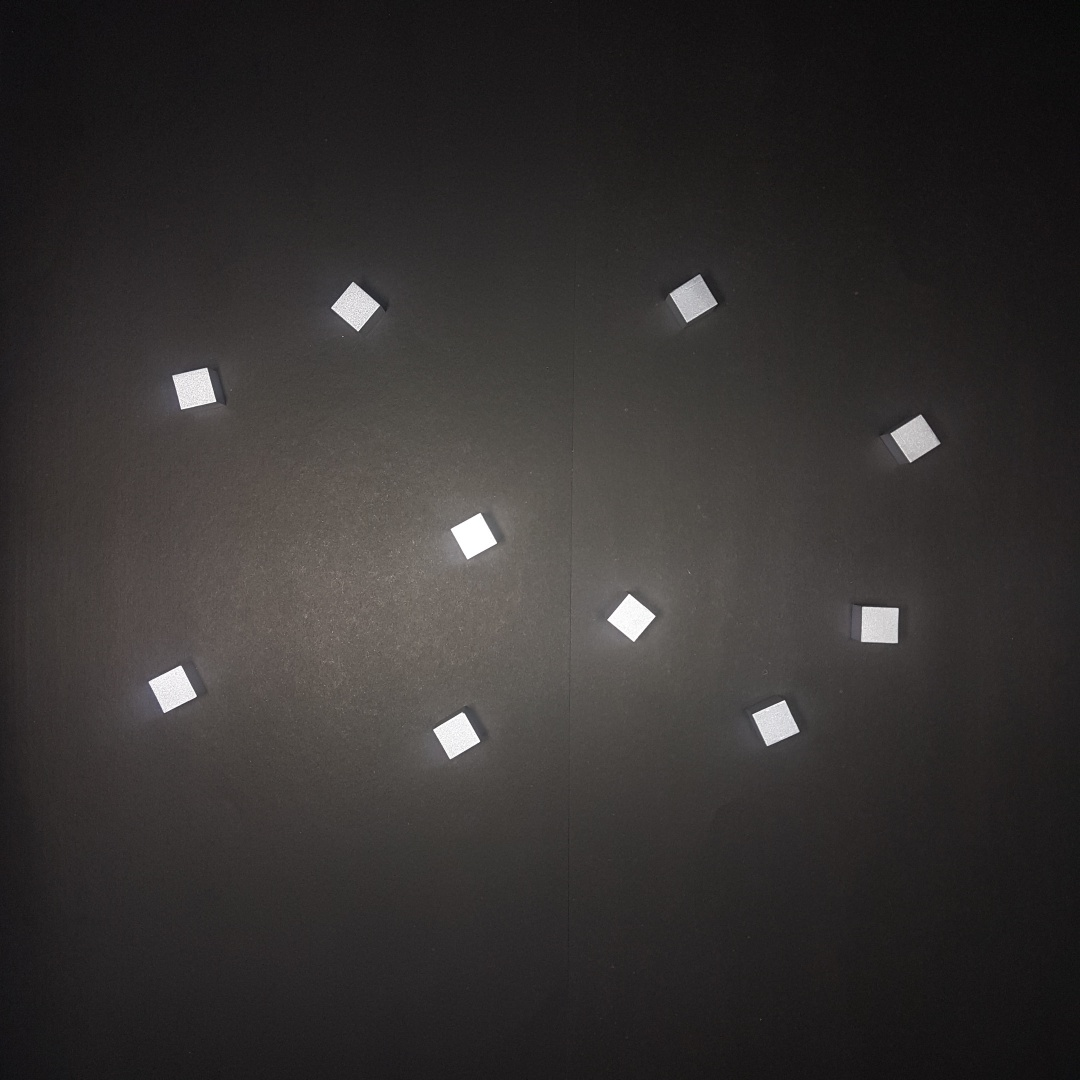
\includegraphics[width=\textwidth]{figures/202106/multiple-cubes.jpg}
         \caption{Top-view of several cubes with bright lighting from above.}
         \label{fig:multiple-cubes}
    \end{subfigure}
    \begin{subfigure}[b]{0.45\textwidth}
         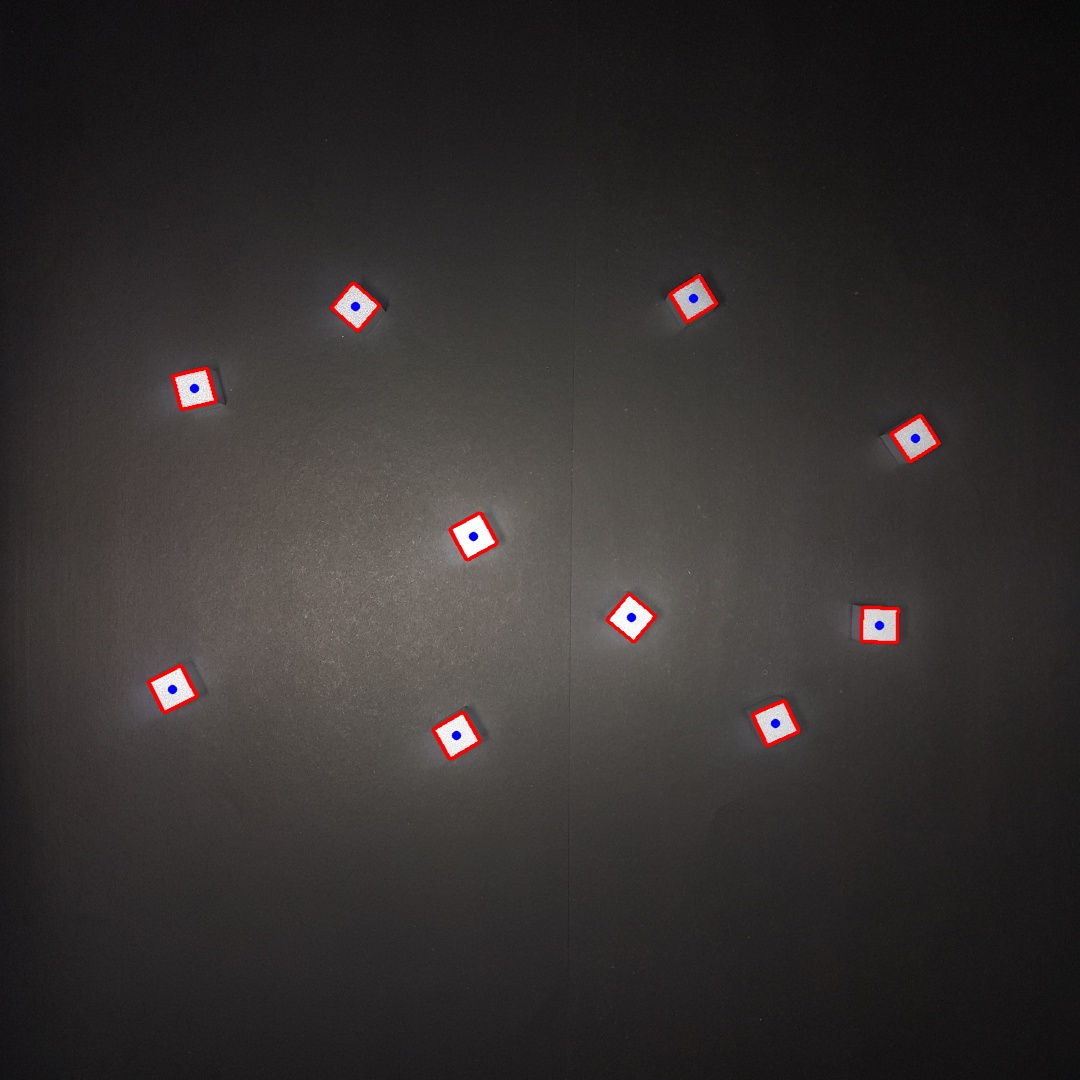
\includegraphics[width=\textwidth]{figures/202106/multiple-cube-centroids.jpg}
         \caption{Output of contour and centroid detection process for cubes in \FigRef{fig:multiple-cubes}.}
         \label{fig:multiple-cube-centroids}
    \end{subfigure}
    \captionsetup{singlelinecheck = false, justification=justified}
    \caption{Centroid detection applied to image containing multiple cubes.}
    \label{fig:multiple-cube-detection}
\end{figure}

\pendsign

